% !TeX spellcheck = en_GB

\subsection{\acrlong{rnn} and \acrlong{lstm}}
\label{subsection:rnn-lstm}

	Human learning does not happen at each moment independently in the sense that every time something new is learned, it depends on the previous knowledge in order to interpret it. This can also be explained by saying that our understanding is persistence.
	
	Traditionally, \acrlong{ann}s have not being able to act in this way. They cannot use time as a property to infer conclusions or predictions from the previous instances that belong to a sequence of data. To address this task, \acrfull{rnn} have been developed, so they can take information and make it persistent. Figure \ref{fig:mesh39} shows a block of a \acrshort{rnn} in which the network, \textit{A}, is fed with an input \textit{x\textsubscript{t}} that is actually a sequence of data. The output is the value \textit{h\textsubscript{t}}. An inner loop takes the information from the outcome and pass it to the input for the next learning step. This can be easily seen in the unrolled part of the right, how the information flows from one element to the next one \cite{Olah2015}. 
	
	\begin{figure}[h]
		\centering
		\captionsetup{justification=centering}
		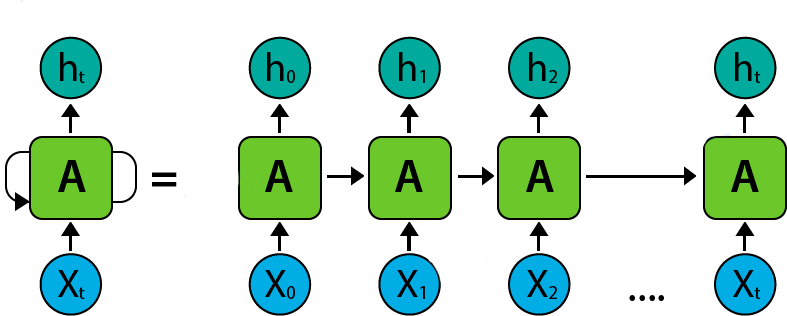
\includegraphics[scale=0.35]{rnn}
		\caption{Scheme or a recurrent neural network about how the loop works }
		\label{fig:mesh39}
	\end{figure}

	This type of networks has became the standard when dealing with sequential data. They have been applied in many tasks, such as language modelling, speech recognition, translation, etc. However, the most simple approach present a problem when the information that must be considering when long-term dependencies. For example, if the task consists of predicting a new instance based on the previous ones in a not really long sequence in which the dependency resides on close instances, normal \acrshort{rnn} can be used and work in the way explained above. When the distance inside the sequence between the predicted element and the ones with the important information that this new one depends on is too large, the network cannot learn this connection \cite{Olah2015}. 
	
	\begin{figure}[h]
		\centering
		\captionsetup{justification=centering}
		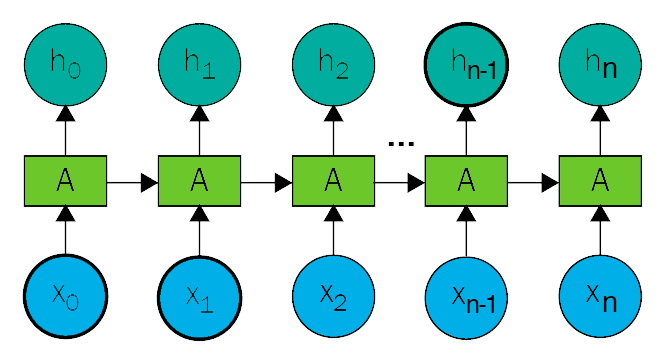
\includegraphics[scale=0.35]{long-term-dependencies}
		\caption{Example of long-term dependencies situation. If the predicted output h\textsubscript{n-1} depends on x\textsubscript{0} and x\textsubscript{1}, the vanishing gradient problem may appear.}
		\label{fig:mesh40}
	\end{figure}
	
	This happens due to the value of the gradients becomes very small during the backpropagation in the learning process. Once the loss function for the new predicted output is calculated, this must be propagated through the rest of the network in order to update the weights. In a typical neural network model, the weights that get updated are those from the hidden layer directly previous to the output one, but, since the data is a sequence, the ones from all the earlier layers must be updated as well. The actual problem appears when renovating the value of the weights through time, i.e. updating the weights used to connect the hidden layers in the unrolled temporal loop. So, if the value of the gradient becomes very small the updating process start to be null when finding the new values of the weights and the model stop learning. This is known as the vanishing gradient problem \cite{SuperDataScienceTeam2018}.
	
	As a solution, a new type of \acrshort{rnn} was developed and named as \acrfull{lstm} networks. These can be defined as a recurrent network that can learn long-term dependencies, so the vanishing gradient problem is not an issue for these models. Nowadays, they are widely used in several fields, since they can remember information along long periods \cite{Olah2015}. The main structure along the model is the same shown above in figure \ref{fig:mesh39}. The difference from the way of working in a common \acrshort{rnn} is the inner architecture in the neural network. In \acrshort{lstm}, the \textit{A} modules are defined as shown in figure \ref{fig:mesh41}. The notation used is as follows: the rectangles denotes a neural network layer, the circle shapes refer to point-wise operations and the arrows means vector transferring.
	
	\begin{figure}
		\centering
		\captionsetup{justification=centering}
		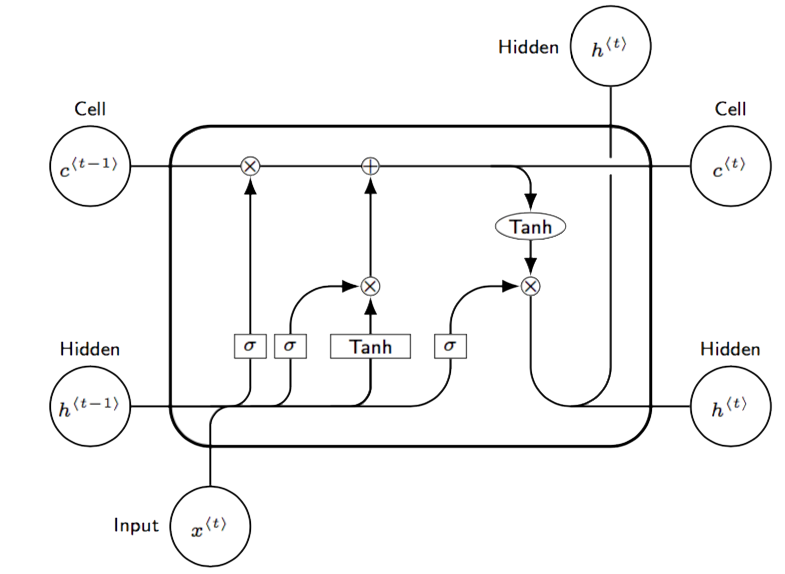
\includegraphics[scale=0.29]{lstm-module}
		\caption{LSTM module with the representation of the different operations that take place inside of it}
		\label{fig:mesh41}
	\end{figure}

	The main concept of a \acrshort{lstm} network resides on its cell state and the different gates. The cell state, represented in the diagram by the upper arrow, is the one in charge of transferring information all the way through the chain of modules. It can be thought as the memory of the whole network. Its objective is to just carry information considered relevant for the model. This way is how the \acrshort{lstm} brings the information from the first layers to the last ones without suffering the vanishing gradient problem. The content of the cell state is modified by the point-wise operations that acts by following the gates criteria. These are in fact neural networks that has the goal of deciding which information can be treated as relevant and so added to cell state. This process can be understood as a learning/forgetting stage \cite{Nguyen2018}. 
	
	\begin{wrapfigure}[9]{l}{0.24\textwidth}
		\centering
		\captionsetup{justification=centering}
		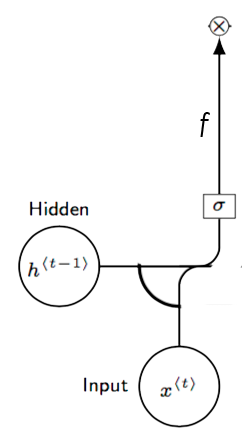
\includegraphics[scale=0.23]{lstm-forget-gate}
		\caption{Forget gate}
		\label{fig:mesh42}
	\end{wrapfigure}

	In order to understanding how this process works, we are going to address the interaction of the different gates in the learning stage.

	The first step is performed by what is called the \textit{forget gate} layer. It must decide which information must be included in the cell state that travels through the time chain. This is why the layer contains a sigmoid function that outputs values between  0 and 1, in which  0 means dropping the information in the previous cell state and 1 implies to keep it. As shown in figure \ref{fig:mesh42}, this is done by paying attention to the hidden state which is the output of the previous module, \textit{h\textsuperscript{<t-1>}}, and the input of the current one, \textit{x\textsuperscript{<t>}} \cite{Nguyen2018}. The resulting function $f$ is defined as follows, where $W_{f}$ are the weights of the \acrshort{rnn} and $b_{f}$ the bias.
	\[
	\ f = \sigma(W_{f}[h^{<t-1>}, x^{<t>}] + b_{f})
	\]
	
	\begin{wrapfigure}{r}{0.28\textwidth}
		\centering
		\captionsetup{justification=centering}
		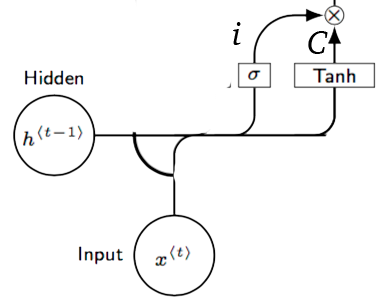
\includegraphics[scale=0.27]{lstm-input-gate}
		\caption{Input gate}
		\label{fig:mesh43}
	\end{wrapfigure}
	
	Next, the decision about what information from the current input \textit{x\textsuperscript{<t>}} must be taken to the cell state is performed. The gate that computes this operation receives the name of \textit{input gate}. This part can be divided into two different steps. First, the previous hidden state, \textit{x\textsuperscript{<t-1>}} ,and the current input feed a \acrshort{rnn} with a sigmoid for the activation function, which takes the decision of which values must be updated by converting them into a range limited by 0 and 1. This result denotes the importance of the value, being 0 non-important and 1, important. Then, also \textit{h\textsuperscript{<t-1>}} and \textit{x\textsuperscript{<t>}} are used as input for the \acrshort{tanh} layer so the values are mapped between -1 and 1. This last activation function is included in order to avoid the vanishing gradient problem previously mentioned, since a function whose second derivative takes more time to tend to zero is needed. Finally, both outputs are multiplied before the updating process in the cell state \cite{Nguyen2018}. The equations for the output of each \acrshort{rnn} module are included below, where $W$ and $b$ denotes the weights and bias for each layer \cite{Olah2015}.
	\[ i = \sigma(W_{i}[h^{<t-1>}, x^{<t>}] + b_{i}) \]
	\[ C = \tanh(W_{C}[h^{<t-1>}, x^{<t>}] + b_{C}) \]
	
	In the step 3, the output of the multiplication from the input gate layer and the output $f$ of the sigmoid function from the forget gate, modify the old cell state from the previous module, \textit{c\textsuperscript{<t-1>}}, so it can be updated. For the outcome of the step 1, a point-wise multiplication is performed, $f * C^{<t-1>}$. Then, to the output of this operation is added the resulting product of the input gate, $i * C$. This two operations can be translated as a forgetting and a learning stage. First, the values the forget gate decided to remove from the cell state are actually forgotten. Then, it must learn the new values belonging to the current input also weighted by their importance, what denotes how much the state values are going to be updated \cite{Olah2015}. The new cell state expression $c^{t}$ is included below and the process is shown in figure \ref{fig:mesh44}.
	
	\begin{wrapfigure}[3]{L}{0.35\textwidth}
		\centering
		\captionsetup{justification=centering}
		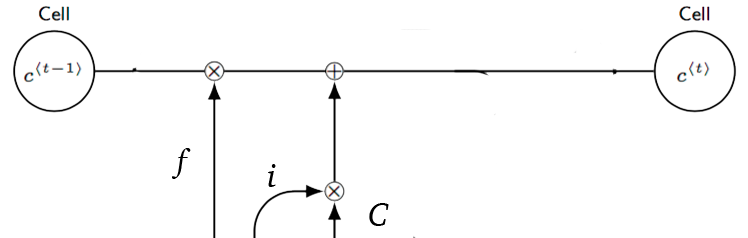
\includegraphics[width=\linewidth]{lstm-cell-state}
		%\vspace{-10pt}
		\caption{Cell state}
		\label{fig:mesh44}
	\end{wrapfigure}
	
	
	\[c^{<t>} = f * C^{<t-1>} + i * C\]
	
				
	Finally, the last step of the module corresponds to the \textit{output gate}. This has the function of deciding how the next hidden state is going to be like. First, \textit{x\textsuperscript{<t>}} and \textit{h\textsuperscript{<t-1>}} are used as input for a layer with a sigmoid activation function and the output $o$ is obtained. Also, the cell state \textit{c\textsuperscript{<t>}} feeds a point-wise \acrshort{tanh} so its values are clipped between -1 and 1. Both outputs are multiplied. The $o$ result decides what values form the current input must be kept in the future hidden state,\textit{h\textsuperscript{<t>}}. The actual output of the module is the hidden state. It also transports the relevant information updated together with the cell state to the next network. The outputs $o$ and $h^{t}$ can be defined as shown below. Also, in figure \ref{fig:mesh45}, the stage of this last part is included.
		
	\begin{figure}[H]
		\ContinuedFloat*
		\[ o = \sigma(W_{o}[h^{<t-1>, x^{t}}] + b_{o}) \]
		\[ h^{<t>} = o * \tanh(C) \]
	\end{figure}

	\begin{figure}[H]
		\centering
		\captionsetup{justification=centering}
		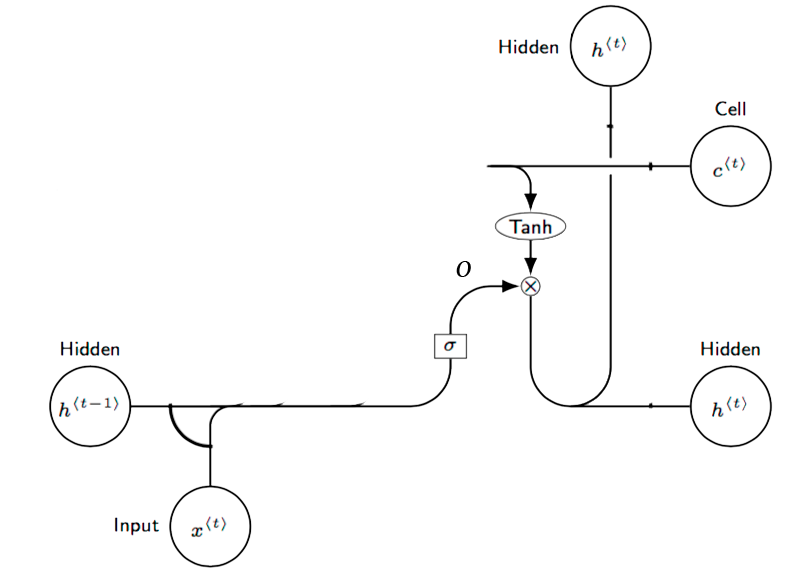
\includegraphics[scale=0.25]{lstm-output-gate}
		\caption{Output gate}
		\label{fig:mesh45}
	\end{figure}

	
	
	
	